\section{Fault Tolerant Algorithm for the QR factorization}
\label{sec:ftla}

To demonstrate the effectiveness of the On-Demand Checkpointing
fault-tolerance mechanism, the QR factorization implementation from
ScaLAPACK~\cite{dongarra1997scalapack} is chosen as the testbed.  QR
factorization is a popular method for solving the linear least squares
problem and QR algorithm which is at the center of a special version
of eigenvalue algorithm. The fault tolerance utilities proposed in
this work can be extended straightforwardly to other linear algebra
operations like LU and Cholesky.

In this section, we first review the fault tolerance QR factorization in ~\cite{lawn253}.
Then the situation where failure occurs during 
lower level routines such as PDLARFB is addressed. Such situation has been
avoided by most of the related work in the area for the compleixty it introduces.
In this work we proposed a novel technique with which failure during 
these lower level routines can be also recovered. 

\subsection{QR factorization on Distributed Memory System}

For an $M\times N$ matrix $A$, QR factorization produces $Q$ and $R$,
such that $A=QR$ and $Q$ is an $M\times M$ orthogonal matrix and $R$
is an $M\times N$ upper triangular matrix.  For simplicity of
expression, we use a square matrix $M\times M$ in this work, but the
result applies also to rectangular matrices. There are several methods
for computing the QR factorization, such as the Gram-Schmidt process,
the Householder transformations, and the Givens rotations. 
\begin{comment}
Today's high
performance math libraries, for instance LAPACK \cite{anderson1999},
ScaLAPACK \cite{choi1996scalapack}, use the Householder
transformations method. 

Given an input matrix $A$, a Householder
matrix $Q_{1}$ is multiplied to $A$ such that
\begin{equation*}
	Q_{1}A=\begin{bmatrix}
		r_{11} & r_{12}\cdots r_{1n}\\ 
		0 &\\
		\vdots  & {A}'\\
		0 &\\ 
	\end{bmatrix}
\end{equation*}
This zeroes out the elements under the diagonal in the first
column. The next step is carried out on the trailing matrix ${A}'$
with
\begin{equation*}
	{Q_{2}}'=\begin{bmatrix}
		1 & 0 & \cdots & 0\\ 
		0 &  &  & \\ 
		\vdots &  & Q_{2}  & \\ 
		0 &  &  & 
	\end{bmatrix}
\end{equation*}
\end{comment}
ScaLAPACK uses a block version of the QR factorization
by accumulating a few steps of the Householder matrix. This method is
rich in level 3 BLAS operations and therefore can achieve high
performance. $Q$ is stored under the lower diagonal of the input
matrix in the form of a $WY$ representation of the Householder
transformation products\cite{schreiber1989storage, bischof1985wy}.

ScaLAPACK implements the block QR factorization as follow. At 
step $i$ , an $m\times m$ submatrix $A_{i}$ is partitioned and
factorized as
\begin{eqnarray*}
A_{i}=\begin{bmatrix}
A_{1} & A_{2}
\end{bmatrix}=\begin{bmatrix}
A_{11} & A_{12}\\ 
A_{21} & A_{22}
\end{bmatrix}
=Q\times \begin{bmatrix}
R_{11} & R_{12}\\ 
0 & R_{22}
\end{bmatrix}
\end{eqnarray*}
Here $A_{11}$ is of size $nb\times nb$, where $nb$ is called the block
size. $A_{21}$ is of size $(m-nb)\times nb$. $A_{1} = [A_{11}, A_{12}]^{T}$
constitutes the area for the panel QR factorization.  Since ScaLAPACK
uses the Householder method, $Q$ is expressed as a series of
Householder transformations in the form $H_{i} =
I-\tau_{i}v_{i}v_{i}^{T}, i=1\cdots nb$.  $v_{i}$ has 0 for the first
$i-1$ entries, 1 on the $i-th$ entry and
$\tau_{i}=2/v_{i}^{T}v_{i}$. In ScaLAPACK, $v_{i}$ is stored below the
diagonal of $A$ and when $Q$ is applied to the trailing matrix
$A_{2}=[A_{21}, A_{22}]^{T}$, $Q$ is computed by $Q=H_{1}\cdots
H_{nb}=I-VTV^{T}$, where $T$ is an upper triangular matrix of size
$nb\times nb$ and $V$ has $v_{i}$ as its $i-th$ column. With this
expression, the trailing matrix update becomes
\begin{eqnarray}
\label{eqn:qr-trailing}
\tilde{A}_{2}=\begin{bmatrix}
\tilde{A}_{12}\\ 
\tilde{A}_{22}
\end{bmatrix}= Q^{T}A_{2}=(I-VT^{T}V^{T})A_{2}
\end{eqnarray}
This finishes one iteration of the block $QR$ factorization. This
process is repeated from $\tilde{A}_{22}$ until the whole matrix is
factorized.

\subsection{Checksum Generation}

\begin{figure}[htb]
	\centering
	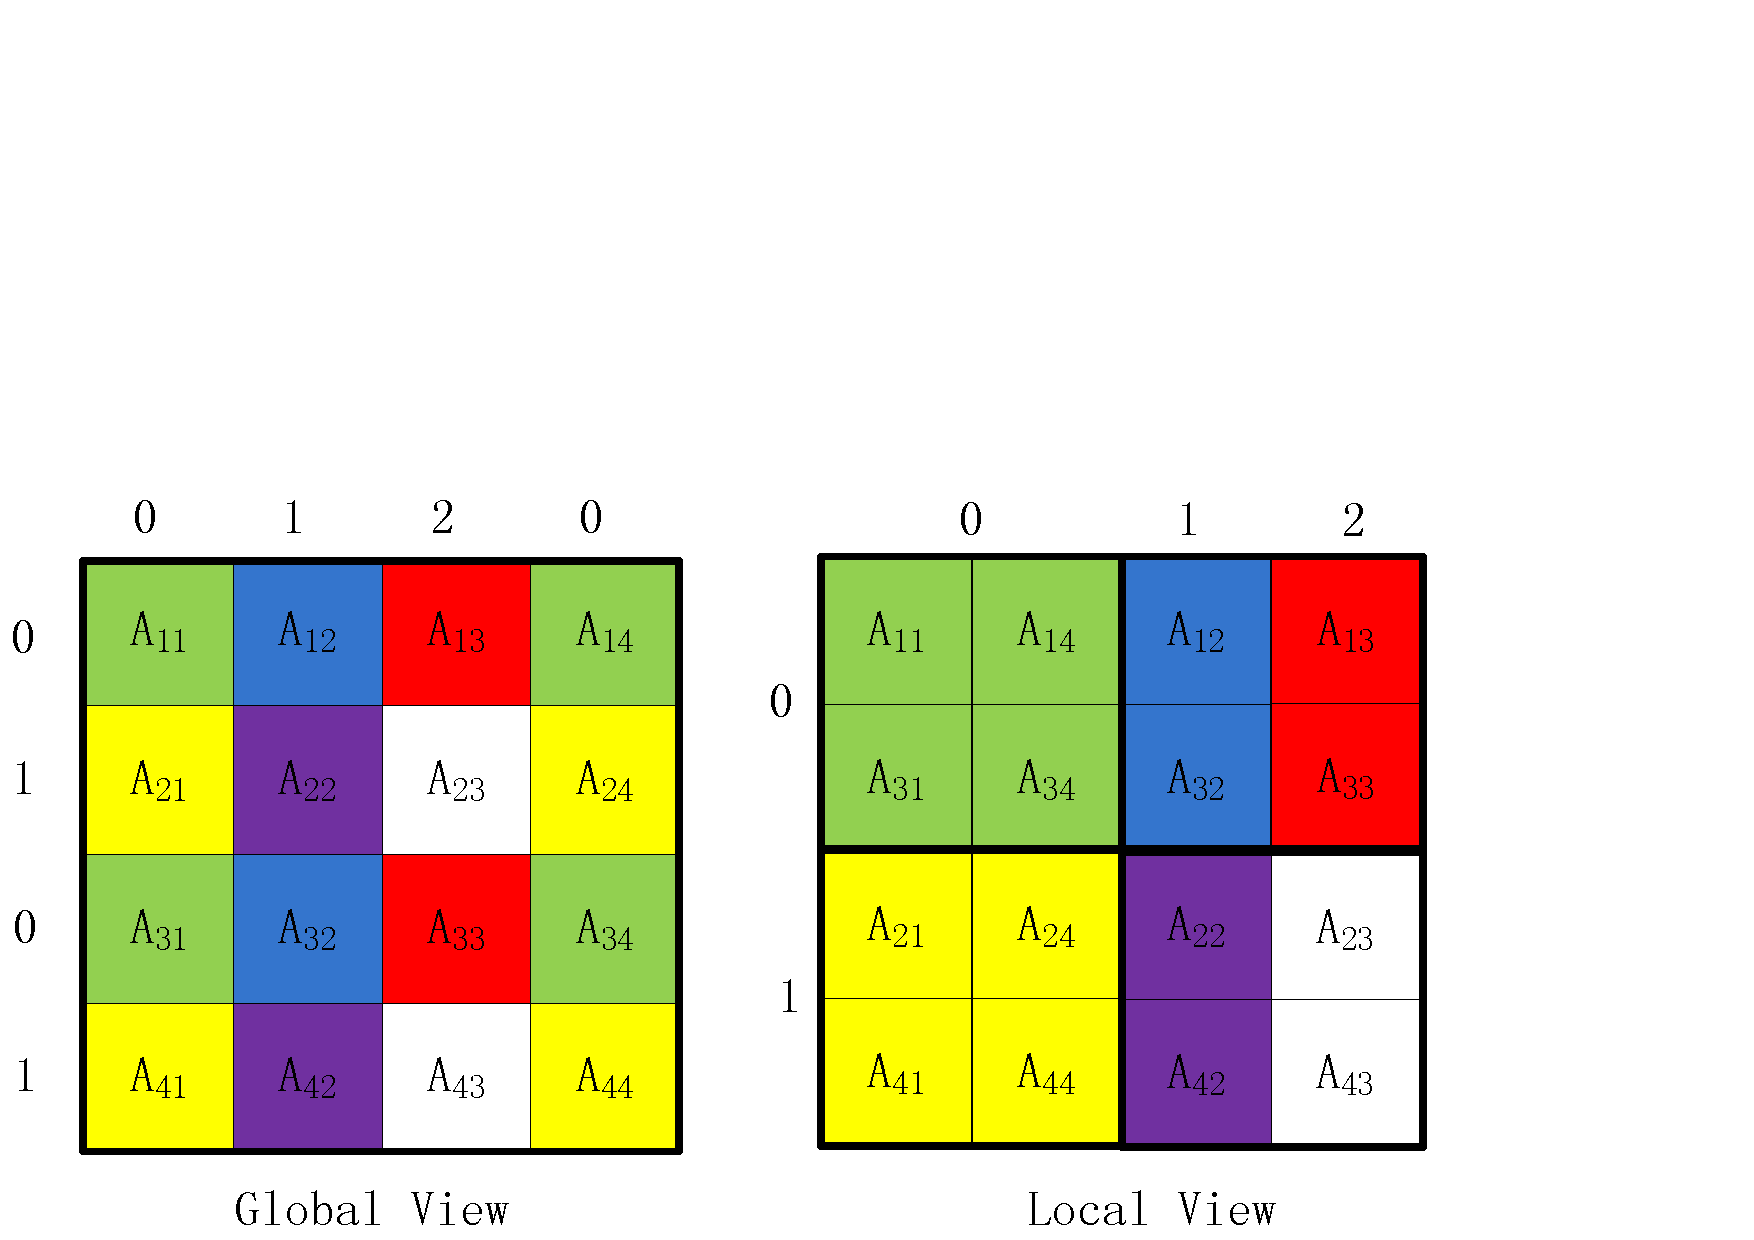
\includegraphics[totalheight=0.15\textheight, width=0.4\textwidth,viewport=1 1 690 360, clip]{figures/2d-block-cyclic}
	\caption{Example of a 2D block-cyclic data distribution}
	\label{fig:2d-block-cyclic}
\end{figure}

For high performance dense matrix factorization, data layout plays a
critical role in the scalability and performance on distributed memory
systems~\cite{choi1996scalapack,kumar1994introduction}. In 2D
block-cyclic distributions, data is split into equally sized blocks,
and all computing units are organized into a virtual two-dimension
grid. Each data block is distributed to computing units in
a round robin fashion, following the two dimensions of the virtual
grid. figure~\ref{fig:2d-block-cyclic} is an example of a $2\times 3$
grid applied to a global matrix of $4 \times 4$ blocks. The same color
represents the same process while numbering in $A_{ij}$ indicates the
location in the global matrix. This layout helps with load balancing
and reduces data communication frequency, since in each step of the
algorithm, many computing units can be engaged in computations
concurrently, and communications pertaining to blocks positioned on
the same unit can be grouped. Because of these advantages, many
prominent software libraries (like
ScaLAPACK~\cite{dongarra1997scalapack}) use a 2D block-cyclic
distribution.

The first step of our algorithm is generating the checksum for the
whole matrix $A$ by $A_{c}=A\times G$, where $G$ is a generator
matrix. This checksum establishes a row-wise summation relationship
between matrix entries and checksum.  However, with a 2D block-cyclic
data distribution, the loss of a single process, usually a computing
node which keeps several non-contiguous blocks of the matrix, results
in holes scattered across the whole matrix. Therefore checksum is
computed for each $M\times (Q\times nb)$ blocks separately.

Let $C_{i}$ be the $i^{th}$ checksum item, and $A_{i}^{j}$, be the
$i^{th}$ data item on process $j$, $\ 1 \leq i \leq \lceil \frac{N}{Q}
\rceil,\ 1 \leq j \leq Q$:
\begin{eqnarray}
\label{eqn:checkpointing}
	C_{k} = \sum_{k=1}^{Q} A_{k}^{k}
\end{eqnarray}

Another issue caused by the 2D block cyclic distribution is that
checksum itself can be lost simultaneously during a failure, if it is
held by the same processor, which renders the \abft recovery
impossible.  To prevent this, a copy of each checksum block column is
made and put on the side of its original column, resulting in $M\times
\left \lceil \frac{2N}{Q} \right \rceil$ storage requirement for
checksum. Compared with the $M\times N$ storage for data, the ratio is
$\frac{2}{Q}$ which becomes negligible when $Q$ is large.

\subsection{Q-parallel Checksum to Protect the Left Factor}

The left factor $Q$ is stored under the lower triangular in the form
of $v$. Since one panel of $v$ of width $nb$ is produced in each
iteration, to protect this portion of data from failure, the
checksum should be generated during the factorization at a regular
interval.  Simple vertical checksum using (\ref{eqn:checkpointing})
that applies vertically on a column suffers from scalability issue
since only up to $P$ processes are involved, and the checksum generation
is on the critical path of LU factorization, depriving the rest
$P\times (Q-1)$ processes of performing trailing update that takes up
most of the computation FLOPS in the factorization. Thus, in this
work, we adopt the scalable $Q$-parallel checksum generation technique
presented in \cite{lawn253} to protect the left factor $Q$.

For the Q-parallel checksum, $P \times Q$ processes are grouped by
sections of width $Q$, called a \emph{panel scope}. When the panel
operation starts applying to a new section, the processes of this
panel scope make a local copy of the impending column and the
associated checksum, called a \emph{snapshot}. This operation features
the maximum $P \times Q$ parallelism due to the fact that all local
copies are performed on each process locally without
communication. The memory overhead involves only the space to keep at
most two extra columns the whole time, one for saving the state before
the application of the panel to the target column, and one for the
checksum column associated to these $Q$ columns. The algorithm then
proceeds as usual, without any further update of the redundant memory
until entering the next $Q$ trailing updates. Because of the
availability of this extra protection column, the original checksum
can be modified to protect the trailing matrix without threatening the
recovery of the panel scope, which can rollback to that previous
dataset should a failure occur.

At the completion of a panel scope, the $P \times Q$ 
processes perform checkpointing simultaneously. Effectively, $P$
simultaneous SUM reduction operations are taking place along the block
rows, involving the $Q$ processes of that row to generate a new
protection block. This scheme enables the maximum parallelism for the 
checksum generation, hence decreasing its global impact on the failure
free overhead.

\subsection{\abft for the Right factor}
The protection of the right factor differs from that of the left
factor because mathematical properties of the algorithm can be utilized 
such that no additional step is needed to keep the checksums up to
date, dropping the necessity of frequently generating checksum to keep
up with the state of the mtraix. 

%lowering the overhead to the initial full-matrix checksum
%generation and extra FLOPS of carrying the checksum columns along with
%factorization.

The use of this technique is illustrated with a $2\times 2$ block
matrix. For an input matrix
\begin{eqnarray*}
A=\begin{bmatrix}
A_{11} & A_{12}\\ 
A_{21} & A_{22}
\end{bmatrix}
\end{eqnarray*}
Checksum is generated using the generator matrix $G$ as 
\begin{eqnarray*}
A_{c}=A\times G=\begin{bmatrix}
A_{11} & A_{12} & A_{13}\\ 
A_{21} & A_{22} & A_{23}
\end{bmatrix}
\end{eqnarray*}

$A_{13}$ and $A_{23}$ are checksum blocks, and
\begin{eqnarray}
\label{eqn:checksum-qr}
\left\{\begin{matrix}
A_{13}=A_{11}+A_{12}\\ 
A_{23}=A_{21}+A_{22}
\end{matrix}\right.
\end{eqnarray}

After performing a QR factorization on $A_{C}$, we have
\begin{eqnarray}
\label{eqn:qrqr}
&&A_{c}=\begin{bmatrix}
A_{11} & A_{12} & A_{13}\\ 
A_{21} & A_{22} & A_{23}
\end{bmatrix}=\nonumber \\
&&\begin{bmatrix}
Q_{11} & Q_{12}\\ 
Q_{21} & Q_{22}
\end{bmatrix}\times
\begin{bmatrix}
R_{11} & R_{12} & R_{13}\\ 
0 &  R_{22} & R_{23}
\end{bmatrix}
\end{eqnarray}

Using Equations (\ref{eqn:checksum-qr}) and (\ref{eqn:qrqr}), the following equation can be obtained:
\begin{eqnarray}
\label{eqn:qr-protect}
&&\begin{bmatrix}
Q_{11} & Q_{12}\\ 
Q_{21} & Q_{22}
\end{bmatrix}\times \begin{bmatrix}
R_{11}+R_{12}-R_{13}\\ 
-(R_{23}-R_{22})
\end{bmatrix}\nonumber \\
&&=Q\times \begin{bmatrix}
R_{11}+R_{12}-R_{13}\\ 
-(R_{23}-R_{22})
\end{bmatrix}=0
\end{eqnarray}

Because $Q$ is non-singular, Equation (\ref{eqn:qr-protect}) can be solved as:
\begin{eqnarray}
\label{eqn:qr-final}
\left\{\begin{matrix}
R_{11}+R_{12}&=&R_{13}\\ 
R_{22}&=&R_{23}
\end{matrix}\right.
\end{eqnarray}

Equation (\ref{eqn:qr-final}) shows that at the end of the QR
factorization, the checksum blocks on the right of the matrix still
hold the same relationship with the data blocks as before the
factorization except only the upper triangular matrix is involved. It
can be further shown that the checksum relationship is also valid
during factorization at the end of each iteration. The proof is beyond
the scope of this paper, but this feature is used to recover lost data
in the right factor at time of failure recovery.

\subsection{Failure in PBLAS routines}
An important condition for the effectiveness of \abft is the
completion of the current iteration. When a failure interrupts the
program execution during an iteration, the checksum ends up in
intermediate form and as a result cannot be used for recovery.  This
problem worsens when a failure occurs during a lower level routine, 
like a PBLAS, causing a partial trailing matrix update. In this case, updates have been applied to parts of the dataset, possibly without having updated accordingly the corresponding checksums. In the case of the QR algorithm, this problem
is solved by saving the local state when a failure is detected in
PDLARFB rather than in PDGEQRF. The recovery
process in this case is described as follow.

\begin{figure}[b]
	\centering
	\subfigure[After the first step: $A_{2}^{T}V$]{\label{fig:gull1}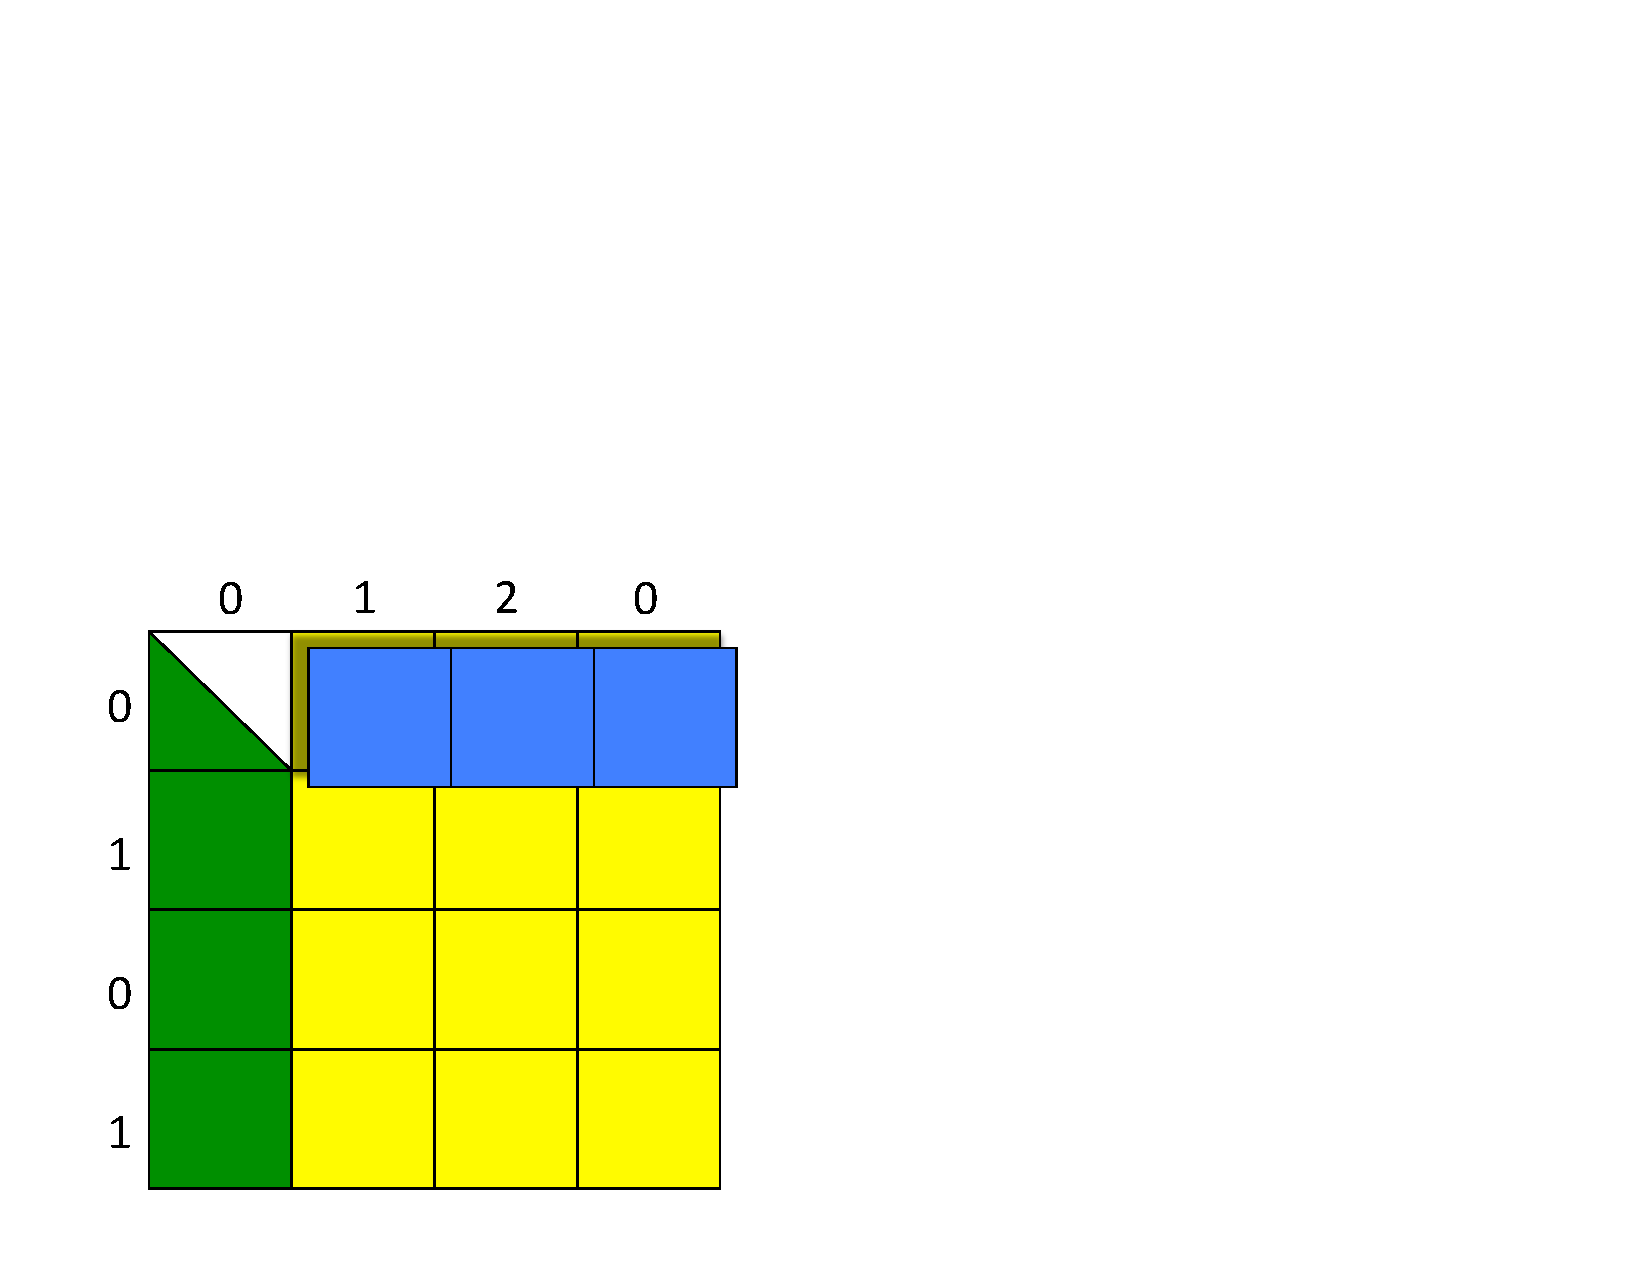
\includegraphics[totalheight=0.15\textheight, width=0.18\textwidth,viewport=10 10 360 360, clip]{figures/pdlarfb_step1}
	\label{fig:pdlarfb_step1}}
	%\line(0,1){100}
	\subfigure[$A_{2}-V\tilde{W}^{T}$]{\label{fig:gull2}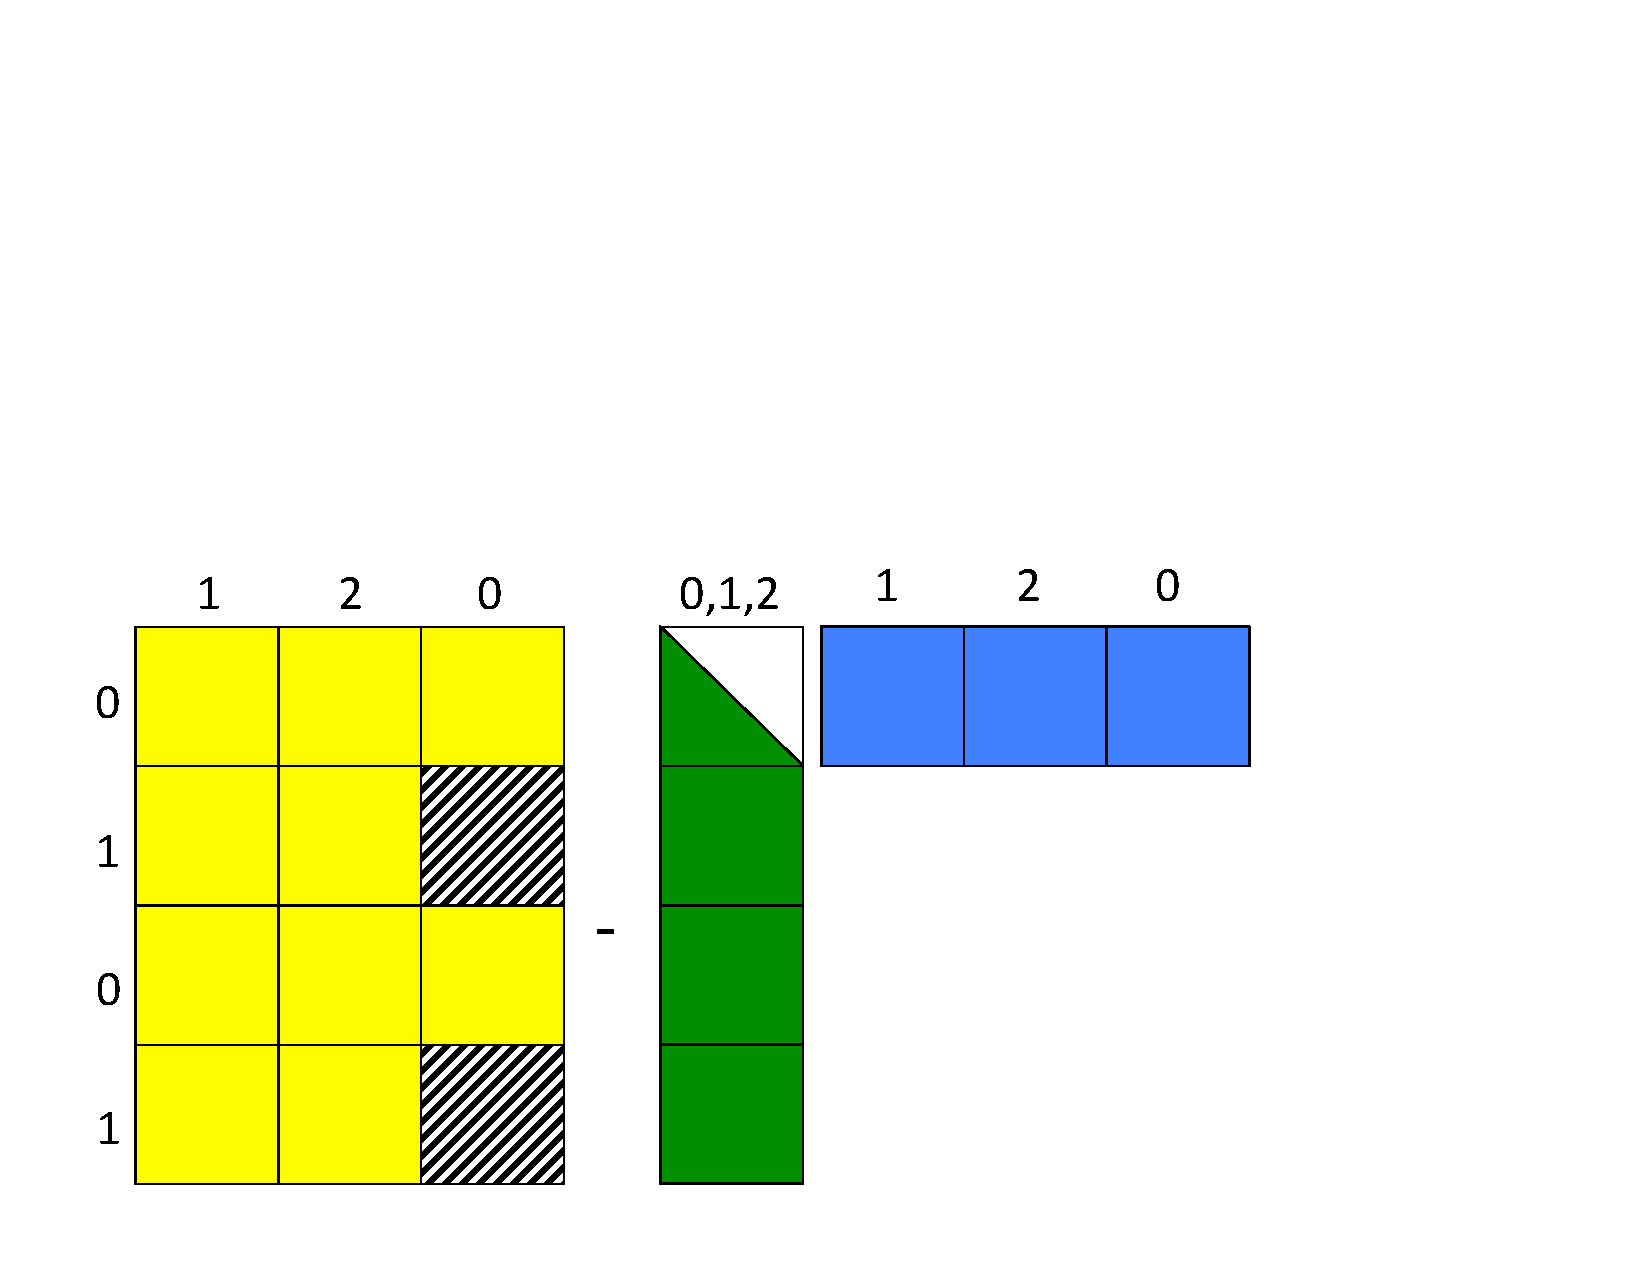
\includegraphics[totalheight=0.15\textheight, width=0.3\textwidth,viewport=10 10 600 360, clip]{figures/pdlarfb_step2}
	\label{fig:pdlarfb_step2}}
	\caption{PDLARFB}
\end{figure}

As shown in Equation (\ref{eqn:qr-trailing}), the trailing update of QR carries
out operation $Q^{T}A_{2}=(I-VT^{T}V^{T})A_{2}\rightarrow
\tilde{A}_{2}$. The right arrow means the updated trailing matrix is
written in-place to $A_{2}$. The trailing matrix update of QR is
similar to PDGEMM for LU which has been shown to hold the checksum
relationship only at the end~\cite{lawn253}. Therefore the procedure
to recover from a failure in PDLARFB is:
\begin{enumerate}
\item Survived processes mark the progress and dump critical data to disk 
\item After re-spawning, all processes dry-run to the failure point
\item All except the replacement process load checkpoint from disk 
\item All processes resume computing from the failure point to the end of PDLARFB
\item At the exit of PDLARFB, recover all lost data in checksum and the whole matrix
\item Execution of PDGEQRF returns to normal
\end{enumerate}
The 'dry-run' step is to re-establish the calling stack of all processes to
the failing point. Therefore PBLAS and ScaLAPACK routines for
computing, for example, PDGEQR2, PDLARFT, etc. are skipped over during 
the dry run.

The recovery is demonstrated with an example of a $4\times 4$ blocks
matrix on a $2\times 3$ grid where failure occurs during PDLARFB.

PDLARFB implements $Q^{T}A_{2}=(I-VT^{T}V^{T})A_{2}$ in three steps:
\begin{enumerate}
\item $W\leftarrow V^{T}A_{2}$
\item $\tilde{W}\leftarrow W\times T$
\item $\tilde{A}_{2}\leftarrow A_{2}-V\tilde{W}^{T}$
\end{enumerate}
Suppose the failure occurs right after step 1 on process (1,0). 
In step 1, as shown in figure~\ref{fig:pdlarfb_step1}, $V$ is stored
in the green trapezoid and $A_{2}$ is in the yellow blocks. $V$ is
first broadcast row-wise to all columns, then GEMM is called on each
process that owns $A_{2}$ with the local $V$ and $A_{2}$. Finally, the
result is produced with column-wise block summation and the result is
stored on the first row of processes that process the first row of
$A_{2}$ (blue blocks).  From the MPI facilities presented in
Section~\ref{sec:mpi}, the failure location is broadcasted to all 
surviving processes and matrix data are dumped to the disk, including
peripheral data like the TAU array and workspace. Surviving processes
also keep a record on whether they have finished the DGEMM in step 1.

After critical data is saved to disk, the program exits and is
re-spawn with a replacement process in the failed process's
location. The re-launched program dry-runs to the failure point in
step 1 of PDLARFB. All previously surviving processes load their
checkpoint from disk while the replacement process stays with its
blank data. Then the program resumes execution of PDLARFB. Since
failure is on process (1,0), $W$ survives the data loss.

Step 2 of PDLARFB is $W\times T$ where $W$ is the blue blocks in
figure~\ref{fig:pdlarfb_step1} and $T$ is a $nb\times nb$ upper
triangular matrix.  Since $T$ resides on each process in the row that
owns $W$, the correctness of $T$ can be always guaranteed, and
therefore $\tilde{W}$ has no lost block in it after calling
DTRMM. $\tilde{W}$ is broadcasted column-wise for step 3.

Step 3 of PDLARFB is shown in figure~\ref{fig:pdlarfb_step2}. In
$\tilde{A}_{2}\leftarrow A_{2}-V\tilde{W}^{T}$, besides
$\tilde{W}^{T}$, $V$ is also correct since $V$ has been broadcast
row-wise to all process in step 1, therefore even if blocks of $V$ are
destroyed by the failure, the result on the replacement process can be
recovered from its neighbour processes in the same row. The result of
step 3, also that of PDLARFB, is affected by the incorrect result in
$A_{2}$, expressed in shadowed blocks in
figure~\ref{fig:pdlarfb_step2}. These incorrect blocks remain in the
result of DGEMM in this step. They are fixed later in the recovery process
in PDGEQRF using both the ABFT and Q-parallel checksum.

For PDLARFB, both $V$ and $T$ can be guaranteed correct no matter when
and where failure occurs, the only variable factor is $W$. However if
the failure does punch holes in $W$, more shadow blocks appear in
the result of PDLARFB, and they can still be fixed by the recovery in
PDGEQRF.
